% Included from both -slides and -handout versions.
\documentclass[pdftex]{beamer} % used to trigger beamer mode in Emacs,
                               % normally commented out.
\usetheme{metropolis}

\usepackage[english]{babel}
\usepackage[latin1]{inputenc}
\usepackage{graphicx}
\usepackage{times}
\usepackage[T1]{fontenc}
\usepackage{fancyvrb}
\usepackage{listings}
\begin{document}
\lstset{language=C, escapeinside={(*@}{@*)}, numbers=left,
  basicstyle=\tiny, showspaces=false, showtabs=false}

\title{Introduction to Operating Systems}
\subtitle{Through tracing, analysis, and experimentation}
%\institute{University of Cambridge}
\author{George V. Neville-Neil}
%\author{Dr Robert N. M. Watson}
\date{1 August 2016}

\begin{frame}
  \titlepage
\end{frame}

\section{Processes}
\label{sec:processes}

\begin{frame}
  \frametitle{The process model}

  \begin{enumerate}
    \item The process model and its evolution
    \item An introduction to virtual memory
    \item Where do programs come from?
    \item Traps and system calls
    \item Reading for next time
  \end{enumerate}
\end{frame}

\begin{frame}
  \frametitle{Review: What is an Operating System?}
  \begin{itemize}
  \item Provider of useful abstractions
  \item Generic interface to varied hardware resources
  \item Controller of resources
  \item Provider of basic security
  \end{itemize}
\end{frame}

\begin{frame}
  \frametitle{Before Processes and Virtual Memory}
  \begin{itemize}
  \item All code in a single address space
  \item No memory protection
  \item Each program must cooperate with all others
  \item Core wars
  \end{itemize}
\end{frame}

\begin{frame}
  \frametitle{What is a process?}
  \begin{itemize}
  \item Container for code
  \item Protective shell between competing programs
  \item \emph{The} defining abstraction on which all modern computing rests
  \end{itemize}
\end{frame}

\begin{frame}
  \frametitle{Process Contents}
  \begin{itemize}
  \item 
  \end{itemize}
\end{frame}

\begin{frame}
  \frametitle{Process Lifecycle}
  
\end{frame}

\begin{frame}
  \frametitle{Scheduling}
  
\end{frame}


\section{The Illusion of Memory}
\label{sec:memory}

\begin{frame}
  \frametitle{The Illusion of Memory}
  \begin{itemize}
  \item How much memory can one process have?
  \item Early UNIX VM systems built on 32 bit hardware.
    \pause
    \begin{itemize}
    \item $4,294,967,296$ bytes
    \end{itemize}
    \pause
  \item Modern systems based on 64 bits.
    \begin{itemize}
    \item $18,446,744,073,709,551,615$ bytes
    \end{itemize}
  \item How does the OS manage this illusion?
  \end{itemize}
\end{frame}

\begin{frame}
  \frametitle{The Purpose of Virtual Memory}
  \begin{description}[labelwidth=\widthof{Simplification}]
  \item [Simplification] Programs (mostly) don't care about addresses.
  \item [Portability] No memory location is more special than any other.
  \item [Protection] All memory accesses go via the kernel.
  \end{description}
\end{frame}

\begin{frame}
  \frametitle{Two Programs in their Virtual Memory Spaces}

  \begin{center}
    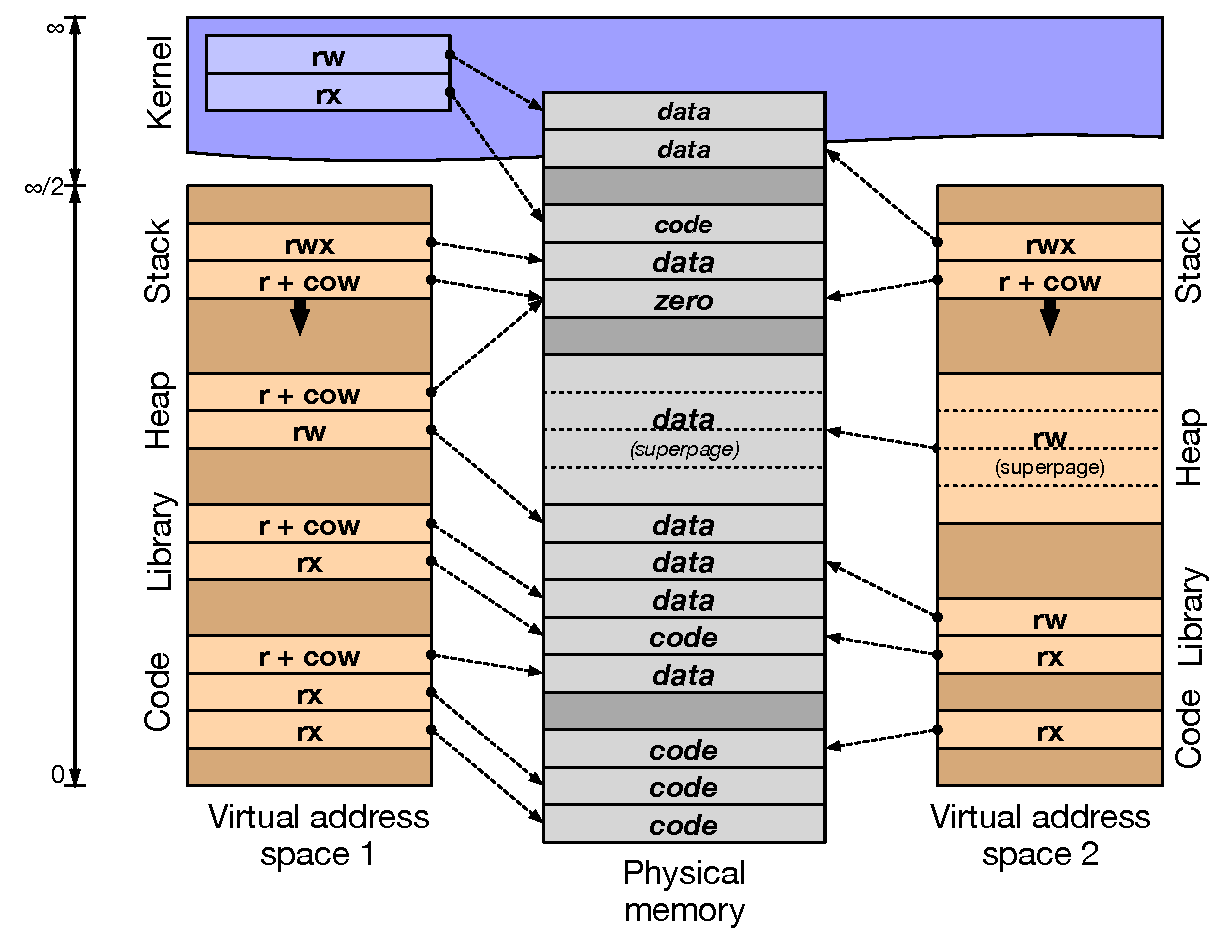
\includegraphics[width=0.8\textwidth]{../../figures/process-address-space.pdf}
  \end{center}
\end{frame}

\begin{frame}
  \frametitle{How does the VM trick work?}

  \begin{itemize}

    \pause

    \item Memory Management Unit (MMU)
    \begin{itemize}
      \item Transforms \textit{virtual addresses} into \textit{physical addresses}
      \item Memory is laid out in \textit{pages} (4K, 2M, 1G...)
      \item Control available only to the supervisor
      \item Software handles failures (e.g., permissions) via traps
    \end{itemize}

    \medskip
    \pause

    \item Page tables
    \begin{itemize}
      \item SW-managed \textit{page tables} provide \textit{virtual-physical
	mappings}
      \item Access permissions, page attributes (e.g., caching)
      \item Various configurations + traps implement BSS, COW, sharing, ...
    \end{itemize}

    \medskip
    \pause

    \item The Translation Look-aside Buffer (TLB)
    \begin{itemize}
      \item Hardware cache of entries -- avoid walking pagetables
      \item Content Addressable Memory (CAM); 48? 1024? entries
      \item TLB \textit{tags}: entries \textit{global} or for a specific process
      \item Software- vs. hardware-managed TLBs
    \end{itemize}

    \medskip
    \pause

%    \item Virtual address spaces
%    \begin{itemize}
%      \item Isolation vs. sharing
%      \item \textit{BSS}, \textit{Copy-on-Write}, \textit{Superpages}
%    \end{itemize}
%
%    \pause

  \end{itemize}
\end{frame}


\end{document}


%%% Local Variables:
%%% mode: latex
%%% TeX-master: "lecture2-processes.tex"
%%% End:
